\documentclass[slidestop,compress,xcolor=table,mathserif,hyperref={bookmarks=false}]{beamer}
%\usetheme{TACC}
\usetheme{boxes}

\usepackage{fancyvrb}
\usepackage{tikz}
\usetikzlibrary{automata,shapes,arrows}
\usepackage{lmodern}
\usepackage[overlay]{textpos}
\usepackage[applemac]{inputenc}
\usepackage{pgfpages}
\usepackage{multirow}

\newenvironment<>{varblock}[2][.9\textwidth]{
  \setlength{\textwidth}{#1}
  \begin{actionenv}#3
    \def\insertblocktitle{#2}
    \par
    \usebeamertemplate{block begin}}
  {\par
    \usebeamertemplate{block end}
  \end{actionenv}}

\author{\textbf{\Large Jim Browne, Leo Fialho and Ashay Rane}}
\begin{document}

\newcommand{\mytilde}{$\sim$}
%------------------------------------------------------------
\pgfdeclareimage[interpolate=true,width=5cm]{logo_TACC}{figures/tacc}
\pgfdeclareimage[interpolate=true,width=5cm]{logo_UT}{figures/ut}
\pgfdeclareimage[interpolate=true,width=1.5cm]{logo_TACC_small}{figures/tacc}
\pgfdeclareimage[interpolate=true,width=1cm]{logo_UT_small}{figures/ut}
\pgfdeclareimage[interpolate=true,width=6cm]{configuration}{figures/configuration}

%------------------------------------------------------------
\title{\textbf{\LARGE Performance Optimization\\for Stampede\\}}
\date{\textbf{\Huge XSEDE 2013} \\ \ \\ \ \\ \pgfuseimage{logo_TACC} \ \ \pgfuseimage{logo_UT}}
\logo{\pgfuseimage{logo_TACC_small} \ \ \ \pgfuseimage{logo_UT_small}}
\frame[plain]{\titlepage}

%------------------------------------------------------------
\section{MACPO}
% \subsection{Agenda}

\frame{\frametitle{Agenda}
	~\\\begin{itemize}
		\item Why another performance tool?\\~\\
		\item What is MACPO?\\~\\
		\item What does MACPO tell you?\\~\\
		\item How to use MACPO?\\~\\
		\item Details of MACPO metrics
	\end{itemize}
}

\frame{\frametitle{State of the art}
	~\\\begin{itemize}
		\item Modern processors can record performance events\\~\\
		\item Performance events provide accurate view of CPU execution\\~\\
		\item Various tools exist to correlate perormance events to user code\\~\\
		\item Ex: PerfExpert, TAU, HPCToolkit, VTune, Scalasca, etc.
	\end{itemize}
}

\frame{\frametitle{But memory is a bigger problem than CPU}
  ~\\\begin{columns}[T]
    \begin{column}{.5\textwidth}
     \begin{block}{}
	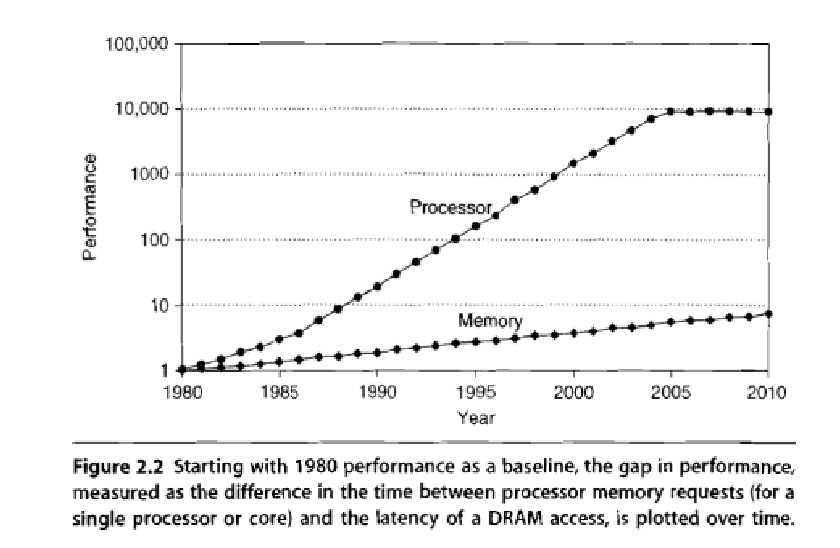
\includegraphics[width=\textwidth]{figures/cpu-mem-speed.eps}\\~\\\tiny Source: Computer Architecture: A Quantitative Approach, 4th Edition by Hennessy and Patterson
% Your text here
    \end{block}
    \end{column}\pause
    \begin{column}{.5\textwidth}
    \begin{block}{}
	\begin{itemize}
		\item For data-intensive applications, application performance usually dependent on memory and not the processor.\\~\\
		\item Performance events provide a CPU-centric, not a memory-centric view.
	\end{itemize}
    \end{block}
    \end{column}
  \end{columns}
}

\frame{\frametitle{Limitations for performance events:\\\#1: Fine-grain measurements}
	~\\\begin{itemize}
		\item Performance events are measured on execution of each instruction\\~\\
		\item \colorbox{blue}{\textcolor{white}{\texttt{mov ah, [1234h]}}} causes cache miss,\\~~~~$\Rightarrow$ increment cache miss counter\\~\\
		\item But memory is optimized for stream traffic and regular accesses (locality, bandwidth, reuse)\\~\\
		\item Hence gap between measurements and optimization techniques
	\end{itemize}
}

\frame{\frametitle{Limitations for performance events:\\\#2: Ambiguous interpretation}
	~\\\begin{itemize}
		\item Same symptoms but different root causes\\~\\
		\item For instance, L3 cache misses could mean any of the following:
		\begin{itemize}
			\item Capacity misses (cold cache)
			\item Poor locality (less reuse of data structures)
			\item False sharing (two processors writing to same cache line)
		\end{itemize}
	\end{itemize}
}

\frame{\frametitle{Limitations for performance events:\\\#3: Little or no scoping}
	~\\\begin{itemize}
		\item Performance events are triggered for all instructions\\~\\
		\item Hence all memory accesses are profiled\\~\\
		\item But information about only specific data structures is desirable\\~\\
		\item Can greatly speed up problem resolution
	\end{itemize}
}

\frame{\frametitle{Hence, MACPO\\\underline{M}emory \underline{A}ccess \underline{C}entric \underline{P}erformance \underline{O}ptimization}
	\begin{itemize}
		\item Analyzes access patterns to find sources of inefficiency\\~\\
		\item Used as part of the compilation process\\~\\
		\item Tracks accesses to arrays and structures within a function\\~\\
		\item Tags each such access with source code location\\~\\
		\item Analyzes accesses to see if access patterns can be improved\\~\\
		\item Works with C, C++ and Fortran code [+ Pthreads, OpenMP]
	\end{itemize}
}

\frame{\frametitle{MACPO workflow}
	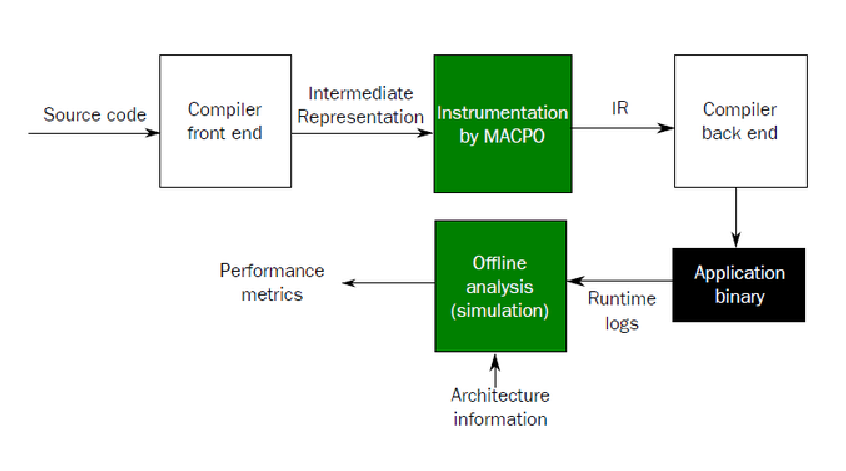
\includegraphics[width=\textwidth]{figures/macpo-workflow.eps}\\
	Combines information from compiler, architecture and simulation
%	\begin{columns}[T]
%		\begin{column}{.5\textwidth}
%	\begin{block}{}
%		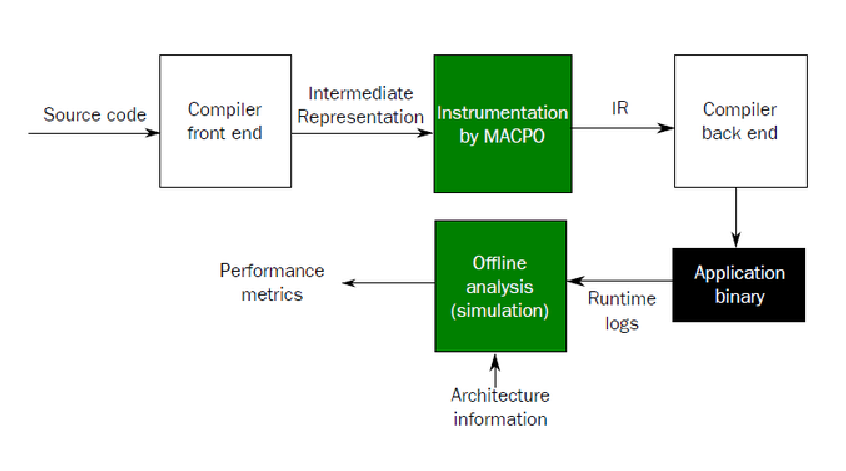
\includegraphics[width=\textwidth]{figures/macpo-workflow.eps}
%	\end{block}
%	\end{column}
%	\begin{column}{.5\textwidth}
%	\begin{block}{}
%		Combines information from compiler, architecture and from simulation
%	\end{block}
%	\end{column}
%	\end{columns}
}

\frame{\frametitle{What does MACPO tell you?}
	~\\For each important variable, MACPO shows:\\~\\
	\begin{itemize}
		\item Access strides and the frequency of occurence\\~\\
		\item Presence or absence of cache thrashing and the frequency\\~\\
		\item NUMA misses\\~\\
		\item Reuse factors for data caches
	\end{itemize}
}

\begin{frame}[fragile]
\frametitle{Sample output}
%\frame{\frametitle{Sample output}
	~\\\scriptsize\begin{Verbatim}[xleftmargin=-7mm]
Var "counts", seen 1668 times, estimated to cost 147.12 cycles on every access
Stride of 0 cache lines was observed 1585 times (100.00%).

Level 1 data cache conflicts = 78.22% [################################        ]
Level 2 data cache conflicts = 63.37% [##########################              ]
NUMA data conflicts = 43.56%          [##################                      ]

Level 1 data cache reuse factor = 97.0% [####################################### ]
Level 2 data cache reuse factor = 3.0% [##                                      ]
Level 3 data cache reuse factor = 0.0% [                                        ]
	\end{Verbatim}
%}
\end{frame}

\frame{\frametitle{How to use MACPO?}
	~\\\begin{itemize}
		\item Compile application using \colorbox{blue}{\textcolor{white}{\texttt{macpo.sh}}}\\~\\
		\item Run application as usual\\~\\
		\item Analyze macpo logs using \colorbox{blue}{\textcolor{white}{\texttt{macpo-analyze}}}
	\end{itemize}
}

\begin{frame}[fragile]
\frametitle{How to use MACPO?}
%\frame{\frametitle{How to use MACPO?}
~\\\footnotesize\begin{verbatim}
# Compile the application using macpo.sh
# Specify code section using --macpo:function or --macpo:loop
$ macpo.sh --macpo:function=thread_func -o mcpi mcpi.cc -lpthread -lrt

# Run the application as usual
$ ./mcpi

# Post-process logs to get analysis output
$ macpo-analyze macpo.out
\end{verbatim}
%}
\end{frame}

\frame{\frametitle{Understanding MACPO metrics}
	~\\\begin{itemize}
		\item Access strides\\~\\
		\item Cache conflicts\\~\\
		\item NUMA misses\\~\\
		\item Reuse factor for data caches
	\end{itemize}
}

\begin{frame}[fragile]
\frametitle{Metric \#1: Cycles per access}
%\frame{\frametitle{Metric #1: Cycles per access}
	~\\Example:\\
	\verb|Var "counts", seen 1073 times,|
	\verb|estimated to cost 8.98 cycles on every access|
	\\~\\\begin{itemize}
		\item Provides esimate of performance impact of accesses to variable\\~\\
		\item Can be used to rule-out variables from further consideration
	\end{itemize}
%}
\end{frame}

\begin{frame}[fragile]
\frametitle{Metric \#2: Access strides}
%\frame{\frametitle{Metric #1: Cycles per access}
	~\\Example:\\
	\verb|Stride of 0 cache lines was observed 983 times (97.62%).|
	\verb|Stride of 2 cache lines was observed 24 times (2.38%).|
	\\~\\\begin{itemize}
		\item Programs that have unit strides or small regular stride values generally execute fast\\~\\
		\item If stide value is high, look for inverted loops affecting the row-major or column-major ordering
	\end{itemize}
%}
\end{frame}

\begin{frame}[fragile]
\frametitle{Metric \#3: Cache conflicts}
%\frame{\frametitle{Metric #1: Cycles per access}
	~\\Example:\\
	\verb|Level 1 data cache conflicts = 78.22%|
	\verb|Level 2 data cache conflicts = 63.37%|
	\\~\\\begin{itemize}
		\item Indicates multiple cores writing to the same cache line\\~\\
		\item Add dummy bytes to the array so that each processor writes to a different cache line
	\end{itemize}
%}
\end{frame}

\begin{frame}[fragile]
\frametitle{Metric \#4: NUMA misses}
%\frame{\frametitle{Metric #1: Cycles per access}
	~\\Example:\\
	\verb|NUMA data conflicts = 43.56%|
	\\~\\\begin{itemize}
		\item NUMA misses generally arise from one processor initializing all of the shared memory\\~\\
		\item To eliminate NUMA misses, have each processor initialize it's portion of shared memory
	\end{itemize}
%}
\end{frame}

\begin{frame}[fragile]
\frametitle{Metric \#5: Reuse factors}
%\frame{\frametitle{Metric #1: Cycles per access}
	~\\Example:\\
	\verb|Level 1 data cache reuse factor = 94.1%|
	\verb|Level 2 data cache reuse factor = 5.9%|
	\verb|Level 3 data cache reuse factor = 0.0%|
	\\~\\\begin{itemize}
		\item Reuse factor indicates the number of times a cache was reused before it was evicted\\~\\
		\item Improve reuse factors by using techniques to improve locality
	\end{itemize}
%}
\end{frame}

\frame{\frametitle{Summary}
	~\\\begin{itemize}
		\item MACPO is a tool to analyze memory access patterns\\~\\
		\item NOT a replacement for PerfExpert. Instead, complements PerfExpert's diagnosis.\\~\\
		\item Allows collection of memory traces for arrays and structures\\~\\
		\item Analyzes traces offline to calculate performance metrics\\~\\
		\item This is an early release, please help us squash the bugs! :)
	\end{itemize}
}

\section{Hands-on MACPO}

\frame{\frametitle{Sample application}
	~\\\begin{itemize}
		\item Monte-Carlo computation of Pi\\~\\
		\item Source code online at: \texttt{http://goo.gl/uEVrh}\\~~~~or at \texttt{{\mytilde}train300/sample-programs.tar.gz}\\~\\
		\item Uses basic C++, parallelized using Pthreads\\~\\
		\item Tasks performed by each thread:
		\begin{itemize}
			\item Generates a buffer of random numbers
			\item For each pair of random numbers, calculates \colorbox{blue}{\textcolor{white}{\texttt{z}}}
			\item Checks a condition on \colorbox{blue}{\textcolor{white}{\texttt{z}}}, based on the result increments a counter
		\end{itemize}
	\end{itemize}
}

\begin{frame}[fragile]
\frametitle{Thread function}
	\begin{verbatim}
int t;
float x, y, z;
thread_info_t* thread_info = (thread_info_t*) arg;
for (int repeat=0; repeat<REPEAT_COUNT; repeat++)
{
  for (int i=0; i<ITERATIONS; i++)
  {
    t = i+thread_info->tid;
    x = random_numbers[t%RANDOM_BUFFER_SIZE];
    y = random_numbers[(1+t)%RANDOM_BUFFER_SIZE];

    z = x*x + y*y;
    if (z < 1) counts[thread_info->tid]++;
  }
}
	\end{verbatim}
\end{frame}

\begin{frame}[fragile]
\frametitle{Commands for sample code}
	~\\\footnotesize\begin{verbatim}
# Extract the source code into the local directory
$ tar -xzf /home1/0003/train300/sample-programs.tar.gz

# Switch to the directory that contains the Monte-Carlo Pi code
cd sample-programs/monte-carlo/

# Compile the application using macpo.sh
# Specify code section using --macpo:function or --macpo:loop
$ macpo.sh --macpo:function=thread_func monte-carlo.cc -o mm -lpthread -lrt

# Run the application as usual
$ ./mm

# Post-process logs to get analysis output
$ macpo-analyze macpo.out
	\end{verbatim}
\end{frame}

\begin{frame}[fragile]
\frametitle{MACPO analysis output (truncated)}
	\begin{verbatim}
$ macpo-analyze macpo.out
	
Var "counts", seen 1668 times,
estimated to cost 147.12 cycles on every access

Stride of 0 cache lines was observed 1585 times (100.00%).

Level 1 data cache conflicts = 78.22%
Level 2 data cache conflicts = 63.37%
NUMA data conflicts = 43.56%

Level 1 data cache reuse factor = 97.0%
Level 2 data cache reuse factor = 3.0%
Level 3 data cache reuse factor = 0.0%
	\end{verbatim}
\end{frame}

\frame{\frametitle{Problem resolution}
	~\\\begin{itemize}
		\item MACPO shows cache thrashing for \colorbox{blue}{\textcolor{white}{\texttt{counts}}} variable.\\~\\
		\item Solution: Add dummy bytes, thus all processors write to different cache lines\\~\\
		\item Optimized code in \texttt{monte-carlo-v2.cc}
	\end{itemize}
}

\begin{frame}[fragile]
\frametitle{MACPO analysis output for optimized code (truncated)}
	\begin{verbatim}
$ macpo-analyze macpo.out
	
Var "counts", seen 1073 times,
estimated to cost 8.98 cycles on every access

Stride of 0 cache lines was observed 983 times (97.62%).
Stride of 2 cache lines was observed 24 times (2.38%).

Level 1 data cache conflicts = 0.00%
Level 2 data cache conflicts = 0.00%
NUMA data conflicts = 0.00%

Level 1 data cache reuse factor = 94.1%
Level 2 data cache reuse factor = 5.9%
Level 3 data cache reuse factor = 0.0%
	\end{verbatim}
\end{frame}

\frame{\frametitle{Review}
	~\\\begin{itemize}
		\item Compiled application using \colorbox{blue}{\textcolor{white}{\texttt{macpo.sh}}}\\~\\
		\item Discovered cache thrashing for the \colorbox{blue}{\textcolor{white}{\texttt{counts}}} array\\~\\
		\item Padding the array reduced cache conflicts from 70\% to 0\%\\~\\
		\item Execution time: 9.14s to 3.17s (65\% improvement)
	\end{itemize}
}

\begin{frame}[fragile]
\frametitle{Summary of MACPO instructions}
	~\\\footnotesize\begin{verbatim}
# Extract the source code into the local directory
$ tar -xzf /home1/0003/train300/sample-programs.tar.gz

# Switch to the directory that contains the Monte-Carlo Pi code
cd sample-programs/monte-carlo/

# Compile the application using macpo.sh
# Specify code section using --macpo:function or --macpo:loop
$ macpo.sh --macpo:function=thread_func monte-carlo.cc -o mm -lpthread -lrt

# Run the application as usual
$ ./mm

# Post-process logs to get analysis output
$ macpo-analyze macpo.out
	\end{verbatim}
\end{frame}

%\frame[plain]{
%	\vspace{3cm}
%	\begin{center}
%		\textbf{\Huge{Thank You}}
%	\end{center}
%	\vspace{2cm}
%	\pgfuseimage{logo_TACC} \ \ \pgfuseimage{logo_UT}
%}

%------------------------------------------------------------
\end{document}
